%%%%%%%%%%%%%%%%%%%%%%%%%%%%%%%%%%%%%%%%%12pt: grandezza carattere
                                        %a4paper: formato a4
                                        %openright: apre i capitoli a destra
                                        %twoside: serve per fare un
                                        %   documento fronteretro
                                        %report: stile tesi (oppure book)
\documentclass[12pt,a4paper,openright,twoside]{report}
%
%%%%%%%%%%%%%%%%%%%%%%%%%%%%%%%%%%%%%%%%%libreria per scrivere in italiano
\usepackage[italian]{babel}
%
%%%%%%%%%%%%%%%%%%%%%%%%%%%%%%%%%%%%%%%%%libreria per accettare i caratteri
                                        %   digitati da tastiera come è à
                                        %   si può usare anche
                                        %   \usepackage[T1]{fontenc}
                                        %   però con questa libreria
                                        %   il tempo di compilazione
                                        %   aumenta
\usepackage[utf8]{inputenc}
%
%%%%%%%%%%%%%%%%%%%%%%%%%%%%%%%%%%%%%%%%%libreria per impostare il documento
\usepackage{fancyhdr}
%
%%%%%%%%%%%%%%%%%%%%%%%%%%%%%%%%%%%%%%%%%libreria per avere l'indentazione
%%%%%%%%%%%%%%%%%%%%%%%%%%%%%%%%%%%%%%%%%   all'inizio dei capitoli, ...
\usepackage{indentfirst}

\usepackage{url}
%
%%%%%%%%%libreria per mostrare le etichette
%\usepackage{showkeys}
%
%%%%%%%%%%%%%%%%%%%%%%%%%%%%%%%%%%%%%%%%%libreria per inserire grafici
\usepackage{graphicx}
%
%%%%%%%%%%%%%%%%%%%%%%%%%%%%%%%%%%%%%%%%%libreria per utilizzare font
                                        %   particolari ad esempio
                                        %   \textsc{}
\usepackage{newlfont}

\usepackage{listings}
\usepackage{algorithmic}
\lstset{breaklines=true
}
%
%%%%%%%%%%%%%%%%%%%%%%%%%%%%%%%%%%%%%%%%%librerie matematiche
\usepackage{amssymb}
\usepackage{amsmath}
\usepackage{latexsym}
\usepackage{amsthm}

%
\oddsidemargin=30pt \evensidemargin=20pt%impostano i margini
\hyphenation{sil-la-ba-zio-ne pa-ren-te-si}%serve per la sillabazione: tra parentesi 
					   %vanno inserite come nell'esempio le parole 
%					   %che latex non riesce a tagliare nel modo giusto andando a capo.

%
%%%%%%%%%%%%%%%%%%%%%%%%%%%%%%%%%%%%%%%%%comandi per l'impostazione
                                        %   della pagina, vedi il manuale
                                        %   della libreria fancyhdr
                                        %   per ulteriori delucidazioni
\pagestyle{fancy}\addtolength{\headwidth}{20pt}
\renewcommand{\chaptermark}[1]{\markboth{\thechapter.\ #1}{}}
\renewcommand{\sectionmark}[1]{\markright{\thesection \ #1}{}}
\rhead[\fancyplain{}{\bfseries\leftmark}]{\fancyplain{}{\bfseries\thepage}}
\cfoot{}
%%%%%%%%%%%%%%%%%%%%%%%%%%%%%%%%%%%%%%%%%
\linespread{1.3}                        %comando per impostare l'interlinea
%%%%%%%%%%%%%%%%%%%%%%%%%%%%%%%%%%%%%%%%%definisce nuovi comandi
%
\begin{document}
\begin{titlepage}                       %crea un ambiente libero da vincoli
                                        %   di margini e grandezza caratteri:
                                        %   si pu\`o modificare quello che si
                                        %   vuole, tanto fuori da questo
                                        %   ambiente tutto viene ristabilito
%
\thispagestyle{empty}                   %elimina il numero della pagina
\topmargin=6.5cm                        %imposta il margina superiore a 6.5cm
\raggedleft                             %incolonna la scrittura a destra
\large                                  %aumenta la grandezza del carattere
                                        %   a 14pt
                             
%
%%%%%%%%%%%%%%%%%%%%%%%%%%%%%%%%%%%%%%%%
\clearpage{\pagestyle{empty}\cleardoublepage}%non numera l'ultima pagina sinistra
\end{titlepage}
\pagenumbering{roman}                   %serve per mettere i numeri romani
\chapter{Lavori Correlati}                 %crea l'introduzione (un capitolo

                                        %   non numerato)
%%%%%%%%%%%%%%%%%%%%%%%%%%%%%%%%%%%%%%%%%imposta l'intestazione di pagina
\rhead[\fancyplain{}{\bfseries
Lavori Correlati}]{\fancyplain{}{\bfseries\thepage}}
\lhead[\fancyplain{}{\bfseries\thepage}]{\fancyplain{}{\bfseries
Lavori Correlati}}
%%%%%%%%%%%%%%%%%%%%%%%%%%%%%%%%%%%%%%%%%aggiunge la voce Introduzione
                                        %   nell'indice
\addcontentsline{toc}{chapter}{Lavori Correlati}
%%%%% Questa \`e l'introduzione \cite{K1} \\
In letteratura esistono diversi studi riguardanti i possibili utilizzi dei dati generati dai sensori degli smartphone, molti dei quali cercano di interpretare i dati generati quando il device si trova a bordo di un veicolo per ottenere informazioni di diverso tipo, come per esempio: determinare il tipo di mezzo di trasporto nel quale si trova lo smartphone \cite{K1, K2, K3, K4} e determinare le condizioni della sede stradale o le condizioni di traffico \cite{K5, K6}. \\

I risultati di questi studi sono interessanti per cercare di ottenere un sistema di navigazione inerziale sempre più efficace (INS, Inertial Navigation System).

\section {Inertial Navigation System}
L' Inertial Navigation System (INS) è un sistema in grado di determinare tramite un meccanismo di Dead Reckoning la posizione di un oggetto in movimento sfruttando esclusivamente i dati raccolti da sensori inerziali.\\

Il sistema è formato da una componente elettronica contenente una serie di sensori (Inertial Measurement Unit, IMU) e da un calcolatore. I sensori rilevano i valori ad una determinata frequenza, l'Inertial Measurement Unit si occupa di inviarli al calcolatore, mediante un qualche sistema di trasmissione dati, che può essere sia cablato che wireless a seconda dell'implementazione fisica del sistema. Il calcolatore elabora i dati e fornisce in output la posizione stimata dell'oggetto. Il calcolatore può essere anche incluso direttamente nell'IMU rendendo il sistema esente da possibili disturbi dovuti alla trasmissione dei dati.

I sensori usati sono esclusivamente sensori inerziali, ossia sensori che basano il loro funzionamento sul concetto del primo principio della dinamica, o principio d'inerzia, il quale afferma che:
\begin{center}
\emph{Un corpo non soggetto a forze esterne, o tale che la risultante delle forze esterne agenti su di esso è nulla, permane nello stato di quiete o di moto rettilineo uniforme, ossia ha un accelerazione nulla.}
\end{center}
Sono, quindi, in grado di rilevare i cambiamenti di stato e le variazioni di moto di un corpo.

I sensori sono: l'accelerometro, il giroscopio e il magnetometro. Il loro funzionamento è esposto nel paragrafo successivo. \\

Il sistema, come detto in precedenza, sfrutta esclusivamente i sensori inerziali, a parte nella fase di inizializzazione.\\
L'inizializzazione consiste nel settare il sistema con tre parametri: la velocità iniziale, l'orientamento iniziale e le coordinate geografiche di partenza. Velocità e posizione di partenza sono dati forniti da strumenti esterni e sono fondamentali per le computazioni successive.\\

L'INS è un sistema ampliamento già usato in ambito marittimo, aeronautico ed aerospaziale. 
In ambito automotive è usato come sistema di navigazione nel caso in cui la tecnologia GPS non sia in grado di funzionare correttamente come nel caso di parcheggi sotterranei, gallerie e in ambito urbano nel caso in cui si percorra una strada in un area piena di edifici che disturbano il passaggio delle onde radio.


\subsection{Dead Reckoning}
Il meccanismo di Dead Reckoning consiste nel determinare la posizione di un corpo in movimento sapendo la posizione di partenza ed altre informazioni come la velocità, direzione e durata dello spostamento.

Possiamo ricondurre questo concetto ad una semplice somma vettoriale. Poniamo la posizione di partenza in un punto nel piano cartesiano, mentre lo spostamento è indicato come un vettore che parte dalla posizione di partenza, che ha come direzione, la direzione dello spostamento mentre come modulo, la distanza percorsa, che ricaviamo dalla velocità e dalla durata dello spostamento.

Nel calcolo della nuova posizione tramite Dead Reckoning [Fig 1.1] bisogna tenere conto dei possibili errori cumulativi generati dai sensori ad ogni nuova computazione. 

Gli errori possono essere causati sia dalla non esatta rilevazione della velocità del moto e da errori nella rilevazione della direzione.

In ambito automotive, ad esempio, se la velocità di un'automobile viene determinata dal numero di rotazioni delle ruote in un'unità di tempo e dalla circonferenza di quest'ultime, a seconda della pressione dei pneumatici, la circonferenza assumerà valori differenti e quindi, di conseguenza, anche la velocità. 
Seppur la differenza tra velocità reale e velocità misurata in un determinato istante può essere molto bassa, quasi ininfluente, nel caso di spostamenti di durata molto alta e quindi con un elevato numero di computazioni di ricalcolo, può risultare importante.
Gli errori dovuti alla non esatta rilevazione della direzione sono causati dalla scarsa precisione dei sensori. Ad esempio, in un tragitto di 1km, la variazione di 1 grado nella direzione porta ad un errore di circa 17,5 metri.


La tecnica del map-matching \cite{K7} è in grado di ridurre questi errori, consiste nell'associare ad ogni nuova posizione calcolata, una posizione reale che corrisponde ad un punto specifico di una strada, si necessità però di una mappa dalla quale ricavare le nuove coordinate.

La posizione del veicolo $(x_k, y_k)$ all'istante $k$ può essere espressa nella seguente maniera \cite{K8}
\begin{center}
$x_k = x_0 + \sum_{i=0}^{k-1} s_i  \cos( \theta_i) $ ,      $y_k = y_0 + \sum_{i=0}^{k-1} s_i  \sin( \theta_i)  $
\end{center}
dove $(x_0, y_0)$ è la posizione iniziale del veicolo al tempo $t_0 $. $s_i$ è la lunghezza del vettore mentre $ \theta_i $ indica il bearing, ossia la direzione del vettore rispetto al nord magnetico.\\
Il bearing relativo è la differenza tra i valori di bearing presi in due istanti consecutivi ed è rappresentata con la lettera $\omega_i $.

Dato il bearing relativo i-esimo $\omega_i$ per ogni istante è facile calcolare $\theta_i$ all'istante $k$:

\begin{figure}[h] 
\centering 
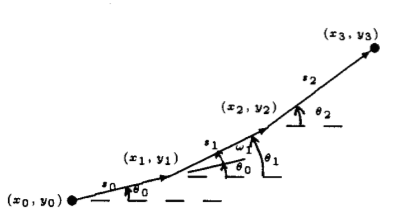
\includegraphics[scale=0.8]{fig1} 
\caption{Dead-Reckoning} 
\end{figure}

\begin{center}
$\theta_k = \sum_{i=0}^k \omega_i$
\end{center}

\section {Sensori}

I sensori disponibili in uno smartphone sono diversi e variano da modello a modello, alcuni sono implementati in maniera hardware (MEMS), altri generano dati mediante algoritmi, quindi in maniera software. 

Nella piattaforma Android possiamo suddividerli in quattro macroaree \cite{K9}:
\begin{itemize}
\item Motion Sensors: include tutti i sensori che misurano le forze di accelerazione e le forze rotazionali come accelerometro, giroscopio, sensore di gravità. Tutte le forze vengono misurate relativamente ai 3 assi.
\item Environmental Sensors: include tutti i sensori che misurano i parametri ambientali come temperatura, pressione atmosferica, illuminazione, umidità. Quindi: termometro, barometro, igrometro e sensore di luminosità.
\item Position Sensors: questi sensori determinano la posizione del device nello spazio come il sensore di orientamento, di prossimità e il magnetometro.
\item Location Sensors: sono indispensabili per la geolocalizzazione del device ed hanno un'accuratezza variabile a seconda della tecnologia, delle condizioni atmosferiche e dalla presenza di ostacoli. Abbiamo: GPS e A-GPS(5m - 10m) \cite{K10}; WIFI e Network Position (10m - 35km).
\end{itemize}

\begin{figure}[h] 
\centering 
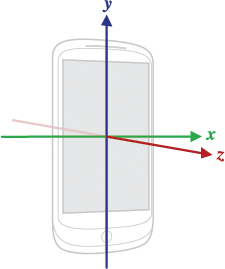
\includegraphics[scale=0.8]{fig2} 
\caption{Sistema delle coordinate} 
\end{figure}

\subsection{MEMS}
MEMS (Micro Electro-Mechanical Systems) è la tecnologia grazie alla quale è possibile realizzare sensori integrati nello smartphone.\\
Un dispositivo MEMS ha un fattore di miniaturizzazione molto elevato, le dimensioni sono davvero contenute, nell'ordine di pochi millimetri di volume.\\
Questo sistema integra dispositivi meccanici, elettrici ed elettronici.\\
La parte meccanica comprende i sensori veri e propri, piccoli chip in grado di misurare fenomeni di natura meccanica, magnetica ed ambientale.\\
Gli elementi meccanici ed elettronici sono integrati in uno substrato di silicio. La parte elettronica del sistema elabora i dati e comunica con lo smartphone. \cite{K14}

\subsection{Accelerometro}
In uno smartphone abbiamo tre accelerometri, ognuno dei quali misura l'accelerazione del device lungo uno dei tre assi. L'unità di misura è $m/s^2$.

\begin{figure}[h!]
\centering 
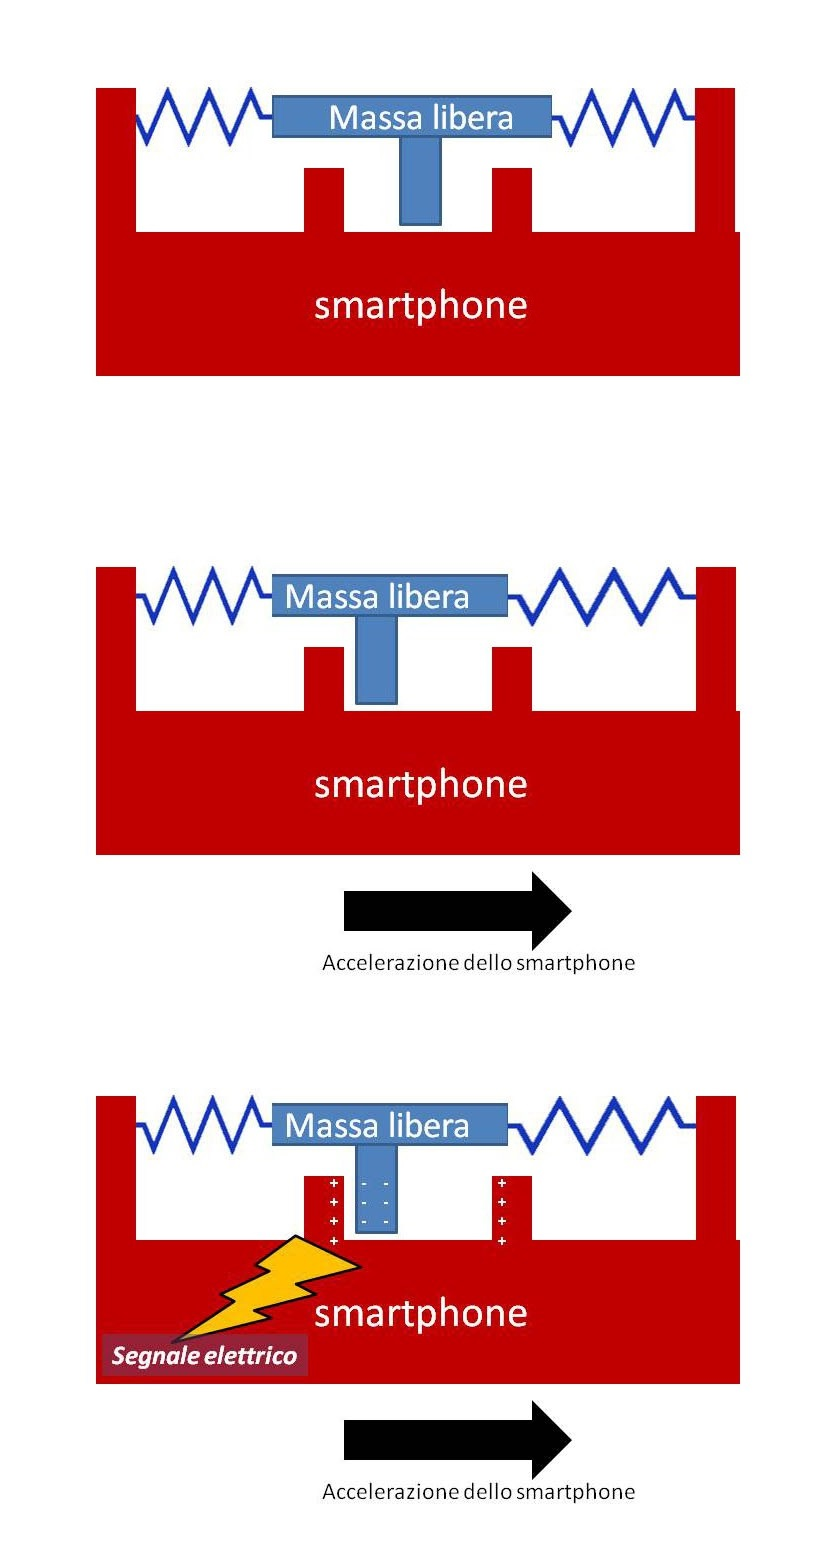
\includegraphics[scale=0.2]{fig4} 
\caption{Accelerometro MEMS} 
\end{figure}
In figura 1.3 possiamo vedere lo schema di funzionamento di un accelerometro MEMS. Abbiamo una massa libera al centro del dispositivo, collegata alle estremità da una molla per parte ad una parte esterna e fissa. Quando c'è un'accelerazione, la massa rimane ferma mentre la parte esterna si muove contraendo le molle e facendo in modo che la massa vada a contatto con le armature dell'accelerometro generando un segnale elettrico. 

Nei valori misurati dall'accelerometro è inclusa la forza di gravità, infatti ponendo lo smartphone su un tavolo vediamo che l'accelerometro relativo all'asse Z rileva un'accelerazione pari a 9,8 $m/s^2$.
Per avere dati esatti bisogna capire anche come è orientato nello spazio il device, tramite il giroscopio e applicare un filtro passa-alto per rimuovere la forza di gravità dai tre assi e isolare quindi l'accelerazione lineare.

Mediante l'accelerometro possiamo determinare accelerazioni e decelerazioni, quindi capire, ad esempio, quando e in che modo un'autovettura frena o accelera e quindi capire anche quando è presente un cambio di velocità del mezzo. 

\subsection{Giroscopio}
Il giroscopio è un dispositivo che misura la velocità angolare del device intorno ai suoi 3 assi. L'unità di misura è $rad/s$. 

Il funzionamento del giroscopio si basa su ciò che afferma la legge di conservazione del momento angolare, la quale afferma che il momento angolare L di un sistema è costante nel tempo se è nullo il momento delle forze esterne che agiscono su di esso.

Per momento angolare si intende il prodotto vettoriale tra il vettore che congiunge un punto del device con un punto dell'asse intorno al quale il device ruota ed il vettore corrispondente alla quantità di moto, ossia $m \cdot v$.
\begin{center}
$\overrightarrow{L} =  \overrightarrow{r} \times \overrightarrow{p}$
\end{center}

\begin{figure}[h!]
\centering 
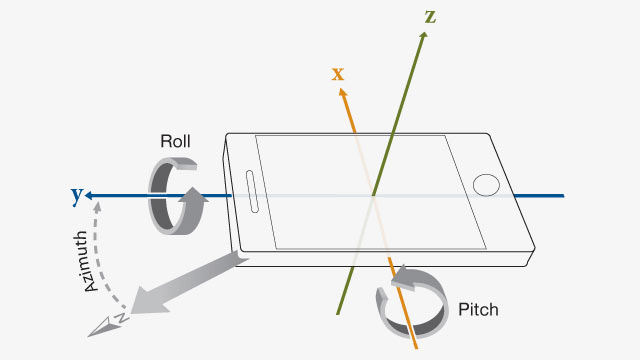
\includegraphics[scale=0.6]{fig6} 
\caption{Giroscopio} 
\end{figure}

Come vediamo nella figura 1.4, l'orientamento del device si può esprimere mediante la velocità rotazionale intorno ai suoi 3 assi, nello specifico, la velocità angolare intorno all'asse x è denominata Pitch, intorno all'asse y è denominata Roll mentre l'orientamento del device rispetto al nord magnetico è denominato Azimuth o Yaw.


Con il giroscopio possiamo determinare l'orientamento del device nello spazio.
E' un tipo di sensore che non molti smartphone posseggono, è possibile, però, simulare il sensore mediante i valori ottenuti dal magnetometro e dalla accelerazione mediante il calcolo delle matrici rotazionali, questo concetto verrà spiegato nel capitolo riguardante l'implementazione del progetto Android.
\subsection{Magnetometro}
Il magnetometro è un dispositivo che misura l'intensità del campo magnetico relativamente ai suoi 3 assi. L'unità di misura è $\mu T$. 


Mediante il magnetometro possiamo determinare la magnitudo del campo magnetico e la direzione del device rispetto al nord magnetico.

\begin{center}
$ magnitude = \sqrt{ x^2 + y^2 + z^2}$
\end{center}
Dove per x,y e z intendo i valori rilevati lungo i rispettivi assi.


\begin{center}
$directionRad = atan2(x,y)$
\end{center}


In questa maniera ottengo la direzione in radianti del device, successivamente trasformo il valore in maniera che il nord magnetico sia a $ \pi / 2$ invece che a 0. Controllo $if directionRad < 0 $ allora $directionRad += 2* \pi $. \\
Infine trasformo il valore da radianti a gradi:

\begin{center}
$directionGrad = directionRad * 180/ \pi$
\end{center}

La magnitudo in un ambiente privo di fonti magnetiche non potrà mai raggiungere lo zero ma si avvicinerà a valori di circa 30-40 $\mu T$, questo è dovuto al campo geomagnetico del pianeta.

\section {GPS}
Il GPS (Global Positioning System) è un sistema di posizionamento satellitare civile gestito dal governo degli Stati Uniti d'America (GSU). Esso permette di ottenere le coordinate geografiche, quindi la geolocalizzazione, di un oggetto.
Ha un livello di accuratezza molto elevato, in ambito militare ha una precisione di circa 1m, in ambito civile di circa 5-10m.

Il sistema è formato da tre segmenti: il segmento spaziale, il segmento di controllo ed il segmento utente. \cite{K15}


Nel segmento spaziale ci sono da 24 a 31 satelliti Navstar che si muovono lungo 6 piani orbitali con una inclinazione di circa 55 gradi rispetto l'equatore,quindi ogni piano orbitale ha 4 satelliti. Da ogni punto della terra sono sempre visibili almeno 4 satelliti, questo in condizioni favorevoli, ossia senza disturbi come edifici o montagne. Ogni satellite dispone di almeno un orologio atomico e trasmette i dati su due frequenze L1(1575,42 Mhz) e L2(1227,60Mhz).


Il segmento di controllo è formato da stazioni di controllo situate in punti diversi del pianeta che si occupano di controllare il funzionamento dei satelliti e degli orologi atomici, la sincronizzazione degli orologi atomici e si occupano della distorsione artificiale (SA, Selective Availability) del segnale per usi civili.


Nel segmento utente fanno parte tutti i dispositivi che fungono da ricevitori GPS.


Il sistema si basa sulla tecnica della trilaterazione. 

\begin{figure}[h!]
\centering 
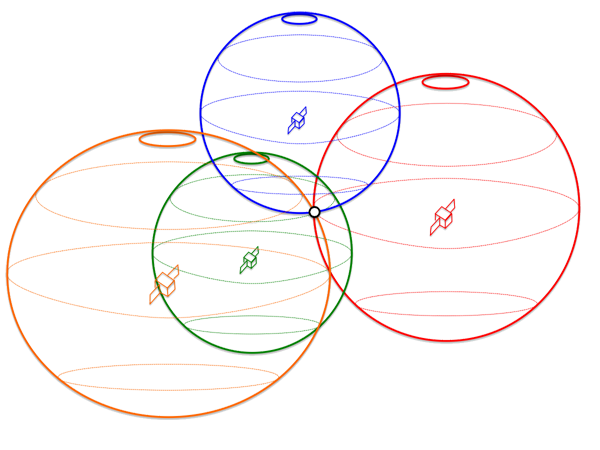
\includegraphics[scale=0.6]{fig8} 
\caption{Punto GPS calcolato mediante 4 satelliti. \cite{K16}} 
\end{figure}
Le coordinate geografiche sono calcolate a partire dal tempo $ \Delta T $ che ci mette il segnale radio a compiere il tragitto satellite-device. Moltiplicando $ \Delta T $ per la velocità della luce otteniamo la distanza. 

Per conoscere la posizione abbiamo bisogno della distanza di almeno 4 satelliti.

\section {Wi-Fi}
Il Wi-Fi è una tecnologia che permette ai dispositivi di trasmettere dati in maniera wireless, quindi senza l'ausilio di cavi. Si basa sulle specifiche dello standard IEEE 802.11.1

Oltre a permettere di accedere ad una rete locale è possibile connettersi tramite un access point ad Internet e trasmettere dati a dei server remoti.

Una rete Wi-Fi può essere identificata tramite il suo SSID (Service Set IDentifier). Il SSID consiste in 32 byte che contengono il nome della rete in formato human-readable. Nel caso un device si connettesse ad una determinata rete, l'SSID può essere utile nel geolocalizzarlo. 
Ad esempio, se un device invia dei dati mediante la rete Wi-Fi Almawifi possiamo dedurre che il device sia nei pressi di una struttura universitaria.\\
Il BSSID, invece, è un identificatore univoco, consiste nel MAC address dell'access point. \\
Il RSSI invece indica l'intensità del segnale, dalla quale possiamo dedurre e stimare la distanza del device dall'access point. L'unità di misura è dBm.

La quasi totalità delle reti private ha dei meccanismi di sicurezza che servono a prevenire accessi da parte di device non autorizzati. 
Abbiamo per esempio WPA (Wireless Protected Access) e WEP (Wired Equivalent Privacy).

\begin{figure}[h!]
\centering 
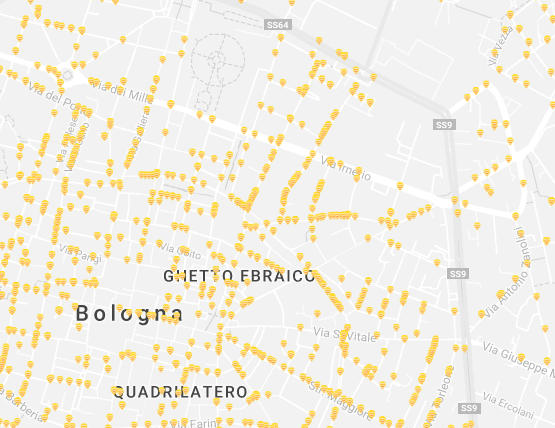
\includegraphics[scale=0.6]{fig7} 
\caption{Hotspot Free a Bologna, dati forniti da fon.com \cite{K16}} 
\end{figure}

Al giorno d'oggi è sempre più facile trovare delle Open-Network \cite{K11}, ossia reti liberi alle quali ci si può collegare gratuitamente. Molti comuni, istituzioni, aree commerciali offrono reti a cui collegarsi liberamente.



\section {OpenStreetMap e Grafi}
OpenStreetMap (OSM) \cite{K12} è un progetto collaborativo open-data che offre un servizio cartografico.\\
OpenStreetMap è stato fondato nel 2004 da Steve Coast e ad ora è usato da molti servizi come Flickr, Strava, WolframAlpha e tanti altri \cite{K13}.

Essendo un progetto open-data è possibile scaricare in locale od usufruire delle API per effettuare query e sviluppare i propri progetti. I dati sono in formato OSM XML.

Gli elementi fondamentali che compongono il \textit{conceptual data model of the physical world} di OpenStreetMap sono:
\begin{itemize}
\item Node: Un nodo consiste in un punto nello spazio, ed è definito da un nodeId univoco, latitudine e longitudine. I nodi possono essere usati per identificare la forma di un edificio o per comporre strade.\\
I nodi possono avere ulteriori tag, come per esempio "highway", "entrance", "natural", etc.\\
I tag sono formati da un insieme di coppie chiave-valore. \\

\begin{figure}[h] 
\centering 
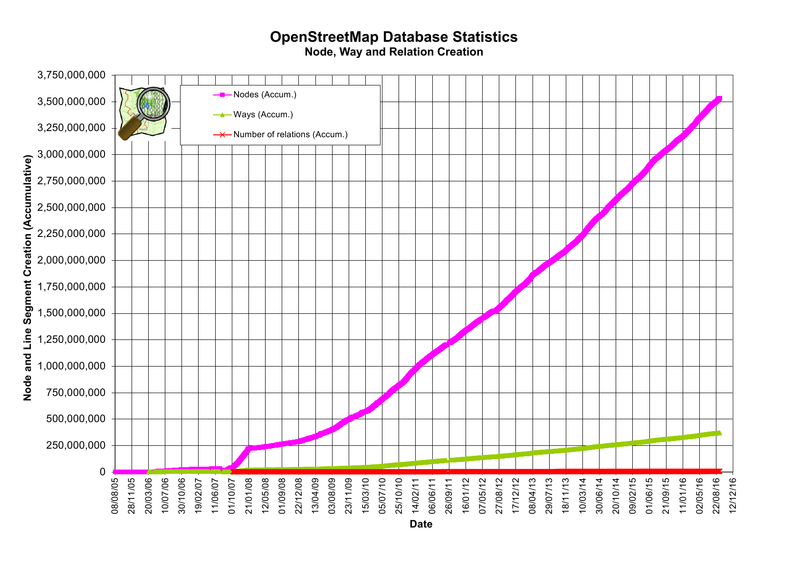
\includegraphics[scale=1]{fig3} 
\caption{Statistiche OpenStreetMap - 2016} 
\end{figure}
\item Way: una way è una lista ordinata di nodi. E' composta da 2 a 2000 nodi. Una way può essere di diversi tipi: chiusa quando l'ultimo nodo è collegato al primo; può essere aperta nel caso di strade; può essere un'area quando delimita una porzione di terreno, se è un area è anche chiusa.\\
Ogni way ha un wayId univoco, una lista di nodi e diversi tag. I più ricorrenti sono "highway", "name", "area", "oneway" e "maxspeed".
\item Relation: una relation è formata da uno o più tags e da un insieme di nodi/way o altre relation che vengono usate per definire relazioni logiche o geografiche tra più elementi. Può essere usata, per esempio, per definire le fermate di un autobus o le stazioni ferroviarie di una determinata linea.
\end{itemize}

\subsection{Grafi}
Un paese, una provincia o addirittura tutto il pianeta può essere inteso come un enorme grafo pesato.
 
Ogni intersezione tra due o più ways può essere vista come un nodo del grafo, mentre una way è appunto la strada che collega due intersezioni è l'edge che collega i due nodi.

Il peso che diamo ad ogni arco può essere o la distanza tra le due intersezioni o il tempo che ci si mette mediamente ad attraversarlo interamente, dipende dai contesti di utilizzo.

In questo modo è facile implementare diversi algoritmi di visita partendo da un nodo di partenza.

Implementando un grafo tramite liste di adiacenza, una DFS (depth-first search) ha una complessità computazionale pari a $\Omega(|V| + |E|) $ dove per $\left|V \right|$ si intende il numero di nodi del grafo e con $\left| E \right|$ il numero di archi.



%%%%%%%%%%%%%%%%%%%%%%%%%%%%%%%%%%%%%%%%%non numera l'ultima pagina sinistra
\clearpage{\pagestyle{empty}\cleardoublepage}



\begin{thebibliography}{90}             %crea l'ambiente bibliografia
\rhead[\fancyplain{}{\bfseries \leftmark}]{\fancyplain{}{\bfseries
\thepage}}
%%%%%%%%%%%%%%%%%%%%%%%%%%%%%%%%%%%%%%%%%aggiunge la voce Bibliografia
                                        %   nell'indice
\addcontentsline{toc}{chapter}{Bibliografia}
%%%%%%%%%%%%%%%%%%%%%%%%%%%%%%%%%%%%%%%%%provare anche questo comando:
%%%%%%%%%%%\addcontentsline{toc}{chapter}{\numberline{}{Bibliografia}}
\bibitem{K1} Widhalm P, Nitsche P, Brandle N. "Transport Mode Detection with Realistic Smartphone Sensor Data". In Proceedings of IEEE CCNC, Las Vegas, USA, 2012; 573-576.
\bibitem{K2} Bedogni L, Di Felice M, Bononi L. "Context-aware Android applications through transportation mode detection techniques". Wirel. Commun. Mob. Comput. 16, 16 (November 2016), 2523-2541.
\bibitem{K3} L. Bedogni, M. Di Felice, L. Bononi, “By Train or By Car? Detecting the User’s Motion Type through Smartphone Sensors Data” on proceedings of the 5th IFIP International Conference Wireless Days 2012 (WD 2012), November 21-23, 2012, Dublin, Ireland
\bibitem{K4} Yu Xiao et al., "Transportation activity analysis using smartphones," 2012 IEEE Consumer Communications and Networking Conference (CCNC), Las Vegas, NV, 2012, pp. 60-61.
\bibitem{K5} R. Bhoraskar, N. Vankadhara, B. Raman and P. Kulkarni, "Wolverine: Traffic and road condition estimation using smartphone sensors," 2012 Fourth International Conference on Communication Systems and Networks (COMSNETS 2012), Bangalore, 2012, pp. 1-6.
\bibitem{K6} Prashanth Mohan, Venkata N. Padmanabhan, and Ramachandran Ramjee. 2008. "Nericell: rich monitoring of road and traffic conditions using mobile smartphones". In Proceedings of the 6th ACM conference on Embedded network sensor systems (SenSys '08). ACM, New York, NY, USA, 323-336.
\bibitem{K7} R. L. French. Map matching origins, approaches and applications. In Second International Symposium on Land Vehicle Navigation, pages 91-116,
Munster, Germany, July 4-7 1989.
\bibitem{K8} Wei-Wen Kao, "Integration of GPS and dead-reckoning navigation systems," Vehicle Navigation and Information Systems Conference, 1991, 1991, pp. 635-643.
\bibitem{K9} \url{https://developer.android.com/guide/topics/sensors/sensors_overview.html}
\bibitem{K10} \url{http://www.gps.gov/systems/gps/performance/accuracy/}
\bibitem{K11} \url{https://openwireless.org}
\bibitem{K12} \url{http://www.openstreetmap.org}
\bibitem{K13} \url{http://wiki.openstreetmap.org/wiki/List_of_OSM-based_services}
\bibitem{K14} \url{http://www.storiaolivetti.it/percorso.asp?idPercorso=575}
\bibitem{K15} \url{http://www1.unipa.it/laser/eln_app/GPS0809.pdf}
\bibitem{K16} \url{https://fon.com/maps/}

\end{thebibliography}

\end{document}
